\section{Results from the simulation}

% \subsection{Overview of the interface}

The simulation, as mentioned above, is articulated in three steps, managed by different windows of the GUI. The first is the generation of the speckle fields, 
the second is the spatial filtering together with caculation of the interference patterns using the resulting filtered speckle fileds, the third is the analysis of 
the patterns and the calculation of the correlation function.

% Maybe add some figures here, illustrating the GUI? Or keep that for the notebook?

% \subsection{Generation of the speckle fields} keep this for the notebook?

\subsection{Interference patterns}

The interference patterns produced look like figure \ref{patt}. In the figure, the modulating function of eqn. \eqref{theopatt} is also shown. Since this 
function is calculated neglecting the effects of partial coherence over each individual slit, the actual pattern has a lower intensity. \\

There are three main effects which in principle have to be taken into account, as can be seen in the figure: 
the modulation of the cosine (due to the finite width of the slits), the loss of visibility (due to the partial coherence between the field amplitudes at the two slits) 
and, as noted above, 
an overall reduction of the intensity if compared with coherent light (due to the partial coherence over the two individual slits). This last feature is accounted 
for by inserting a multiplicative constant as an additional parameter in the fit.
\begin{figure}[!ht]
    \centering
    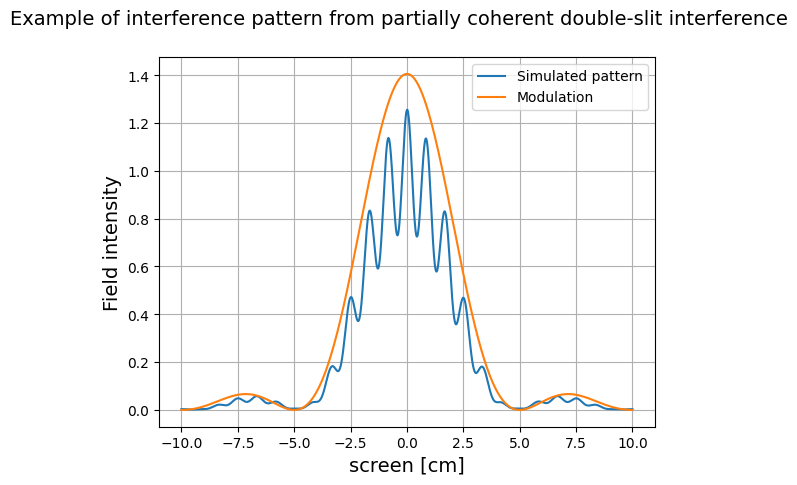
\includegraphics[width = .8\textwidth]{Img/output.png}
    \caption{Typical interference pattern}
    \label{patt}
\end{figure}

\subsection{Data analysis}

The interface for data analysis allows to automatically compute the visibility of each interference pattern (previously generated and stored as csv files) as 
a function of either the width of the spectral density after the spatial filtering, or the separation between the slits. In the latter case, the resulting 
function is exactly the absolute value of the normalized field correlation function, as per eqn. \eqref{vis_formula}: this allows to calculate the correlation 
length $\Delta l$ as the FWHM (or another width measure) of the correlation function. The dependence on the spectral density width $\Delta k$ allows then to 
verify the inverse proportionality between $\Delta l$ and $\Delta k$. \\

The automatic analysis of all the interference patterns is carried out by first dividing each one by the modulating function, suitably normalized, in order 
to obtain a nearly (co)sinusoidal pattern (like in figure \ref{data_an_2}); the visibility can then be calculated using eqn. \eqref{vis_formula}. 
It is also possible to consider an individual pattern at a time: in this case, the interface allows to choose the initial parameters in order to perform a 
fit of both the upper and lower profile of the interference pattern (the local maxima of the pattern belong to the upper profile and the local minima belong 
to the lower pattern). This is shown in figures \ref{data_an_1} and \ref{data_an_2}

\begin{figure}[!ht]
    \centering
    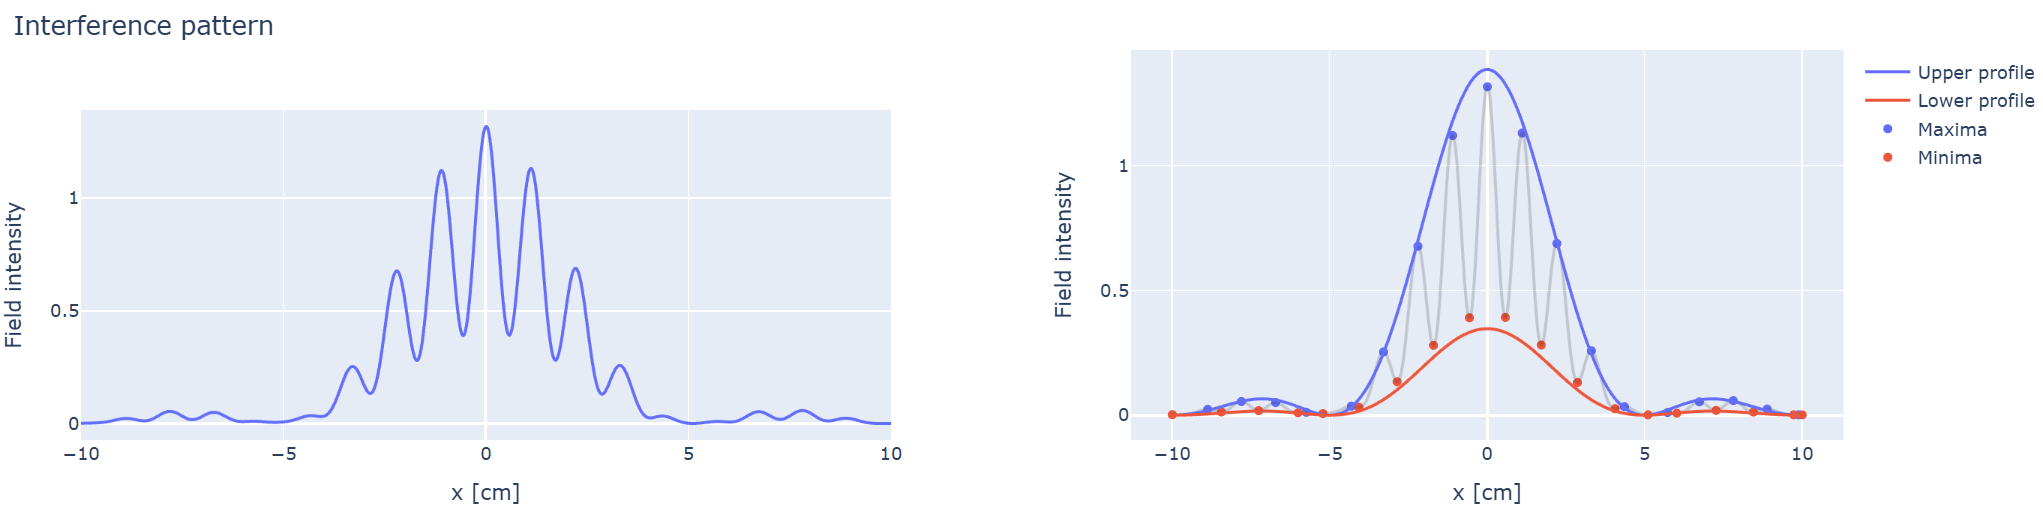
\includegraphics[width = \textwidth]{Img/an_11.png}
    \caption{Data analysis interface}
    \label{data_an_1}
\end{figure}

\begin{figure}[!ht]
    \centering
    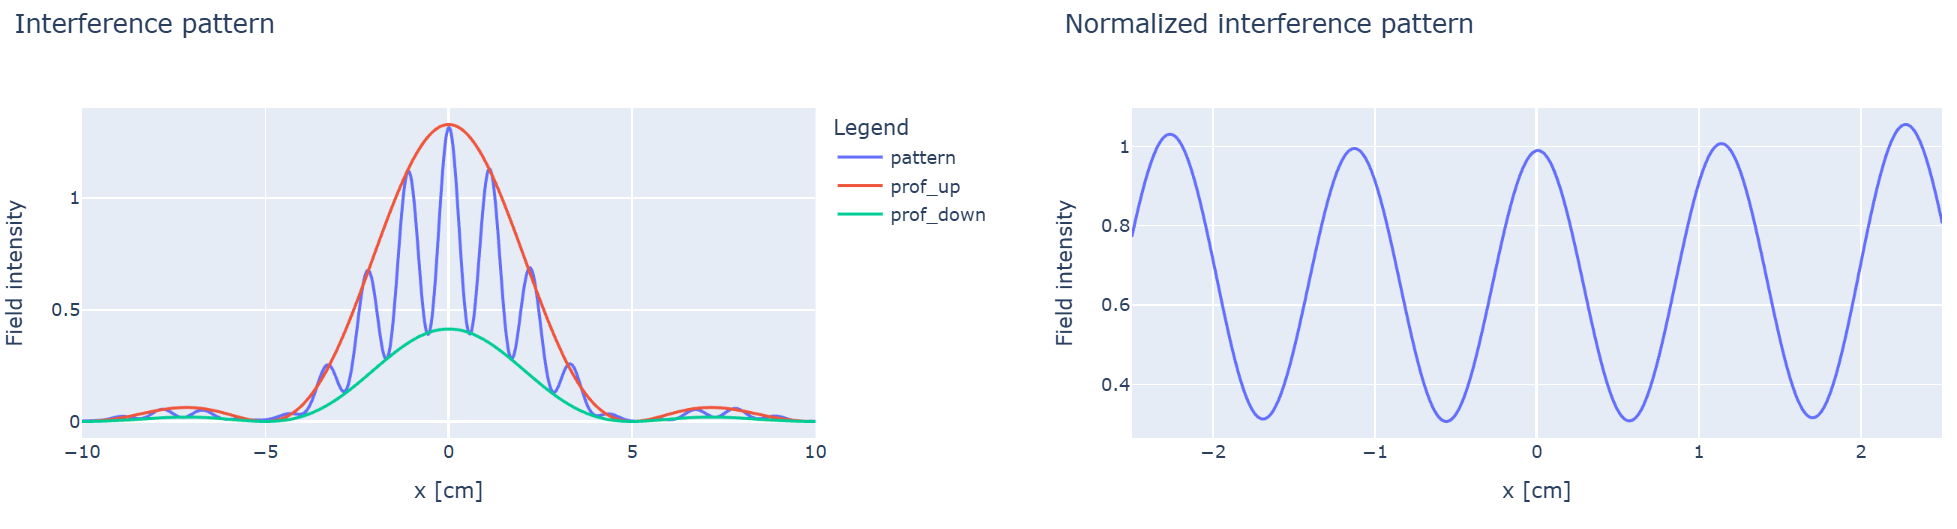
\includegraphics[width = \textwidth]{Img/an_22.png}
    \caption{Data analysis interface}
    \label{data_an_2}
\end{figure}

